%%%%%%%%%%%%%%%%%%%%%%%%%%%%%%%%%%%%%%%%%%%%%%%%%%%%%%%%%%%%%%%%%%%%%%%%%%%%%%%%%%%%%%%%%%%%%%%%%%%%%
%%%%%%%%%  1. Mose
%%%%%%%%%%%%%%%%%%%%%%%%%%%%%%%%%%%%%%%%%%%%%%%%%%%%%%%%%%%%%%%%%%%%%%%%%%%%%%%%%%%%%%%%%%%%%%%%%%%%%
\section{1. Mose (Genesis)}
\subsection{WER?}
Als Autor wird Moses erwähnt. Dies wird in mehreren Schriftstellen in der Bibel bestätigt.
\utitle{Aus dem Alten Testament: }
\begin{bibeltext}{Sch2}{Ex}{17:14}
	Da sprach der \herr{} zu Mose: \textquote{Schreibe das zum Gedenken in ein Buch und präge es den Ohren Josuas ein: Ich will das Andenken Amaleks ganz und gar austilgen unter dem Himmel.}
\end{bibeltext}
\begin{bibeltext}{Sch2}{Num}{33:2}
    Und Mose schrieb ihren Auszug und ihre Tagereisen auf Befehl des \herr{} nieder.
\end{bibeltext}

\begin{bibeltext}{Sch2}{Neh}{13:1}
    Zu jener Zeit wurde den Ohren des Volkes im Buch Moses gelesen und darin geschrieben gefunden, dass kein Ammoniter und Moabiter in die Geneinde Gottes kommen sollte ewiglich.
\end{bibeltext}
\utitle{Aus dem neuen Testament: }
\begin{bibeltext}{Sch2}{Mt}{8:4}
    Und Jesus spricht zu ihm: \textquote{Sieh zu, dass du es niemand sagst; sondern geh hin, zeige dich dem Priester und bringe das Opfer dar, das Mose befohlen hat, ihnen zum Zeugnis!}
\end{bibeltext}
\begin{bibeltext}{Sch2}{Joh}{5:14}
    Danach findet ihn Jesus im Tempel und spricht zu ihm: \textquote{Siehe, du bist gesund geworden; sündige hinfort nicht mehr, damit dir nicht etwas Schlimmes widerfährt!}
\end{bibeltext}
\begin{bibeltext}{Sch2}{Rom}{10:19}
    Aber ich frage: \textquote{Hat es Israel nicht erkannt? Schon Mose sagt: \textquote{Ich will euch zur Eifersucht reizen durch das was kein Volk ist; durch ein unverständiges Volk will ich euch erzürnen}}
\end{bibeltext}
\begin{bibeltext}{Sch2}{2Kor}{3:15}
   Doch bis zum heutigen Tag liegt die Decke auf ihrem Herzen, sooft Mose gelesen wird. 
\end{bibeltext}
In diesen Bibletexten wird bestätigt, dass das die Bücher Mose von Moses selber geschrieben wurde. Auf Grund seiner hohen Stellung im Hofe des Pharao hat er eine Bildung genossen, die ihm das Schreiben ermöglichte. Bis jetzt wurde noch keine Beweise aufgeführt oder gefunden, die Mose als Verfasser widerlegen.
\subsection{WEM?}
Eigentlich wurde das Buch für die ganze Menschheit geschrieben. Das erste Buch Mose (Genesis) bezeugt, dass Gott existiert. Dies wir schon im ersten Satz des ersten Kapitel erwähnt:
\begin{bibeltext}{Sch2}{Gen}{1:1}
    Im Anfang schuf Gott die Himmel und die Erde.
\end{bibeltext}
Es gibt keine Anzeichen, dass Gott irgendwie entstanden ist. Der \herr{} war schon immer. Er ist der Anfang und das Ende. Das $\alpha$ und das $\Omega$.
Die Bücher Mose wurden in erster Linie für Israel geschrieben. Dies sag der \herr{} auch Josua im ersten Kapitel.
\begin{bibeltext}{Sch2}{Jos}{1:8}
   Lass dieses Buch des Gesetzes nicht von deinem Mund weichen, sondern erforsche darin Tag und Nacht, damit du darauf achtest, alles zu befolgen, was darin geschrieben steht; denn dann wirst du Gelingen haben auf deinen Wegen, und dann wirst du weise handeln. 
\end{bibeltext}
Das erste Buch Mose enthält die Geschichte der Welt und vom Volk Israel und die restlichen viel Teile beinhalten die Gesetzte und Anweisung von Gott an das Volk Israel.
\subsection{WANN?}
Die Bücher Mose sind wohl gegen Ende der Wüstenwanderung geschrieben worden. Der Auszug aus Ägypten wird ca. 1445 v.Chr. datiert. Moses Tod war um die Zeit 1405 v.Chr.. Irgend wann in dieser Zeit wurden die 5 Bücher geschrieben. Das erste Buch Mose wurde wohl zu beginn des Exodus geschrieben.
\subsection{WAS?}
Das erste Buch Mose umfasst 2000 Jahre Urgeschichte. Sie beginnt bei der Schöpfung und endet mit Tod Josef in Ägypten. 400 Jahre danach erscheint dann Mose.
Das erste Buch ist in zwei Teilen unterteilt und diese jeweils wieder in vier Unterteile. Schon im ersten Buch der Bibel kann man den Heilsplan Gottes erkennen. Nach dem Sündenfall des Menschen, beginnt ein systematischer Plan Gottes um die Menschen wieder auf den richtigen Weg in seine nähe zu kriegen. Dieser Heilsplan die Erlösung, d.h. die Rückführung des Menschen zu Gott durchzieht die Schrift wie ein roter Faden
\begin{enumerate}
    \item \textbf{die Urgeschichte \hspace{1cm} \bibleverse{Gen} {1-11}}
    
    \begin{tabular}{cll}
        1.&die Schöpfung &\bibleverse{Gen} {1-2} \\
        2.&der Sündenfall &\bibleverse{Gen} {3-5} \\
        3.&die Sintflut &\bibleverse{Gen} {6-9} \\
        4.&die Sprachenverwirrung&\bibleverse{Gen} {10.11}\\ 
    \end{tabular}
    \item \textbf{die Patriarchengeschichte \hspace{1cm} \bibleverse{Gen} {1-11}}
    
    \begin{tabular}{cll}
        1.&Abraham& \bibleverse{Gen} {12;1-25;8}\\
        2.&Isaak &\bibleverse{Gen} {21;1-35:29}\\
        3.&Jakob &\bibleverse{Gen} {25;21-50;14}\\
        4.&Josef &\bibleverse{Gen} {30;22-50;26}\\
    \end{tabular}
\end{enumerate}
\subsection{WIE?}
Der erste Teil ist erzählend aufgeschrieben. Es ist die Geschichte der Menschen aufgeschrieben. Der Teil vor der Sintflut und dann nach der Sintflut. Nach der Sintflut hat sich die Welt verändert. Die Erde wurde anders die Menschen wurden jünger. Was sich aber nicht geändert hat ist der Mensch selber. Auch nach der Sintflut blieb er rebellisch und Gott fern.

Theologisch kann viel von den Patriarchen gelernt werden. Auch die Geschichte von Josef in Ägypten ist bemerkenswert und ist immer noch aktuell. Diese zeigt auf das Gott für jeden Menschen seinen Plan hat. Auch für uns. Da wir mitten drin sind sehen wir selber das nur schwer. Ich glaube so richtig klar wird es uns dann erst nach dem Tod.
\subsection{Übersichtsfragen zu 1. Mose}
    
\begin{enumerate}
    \item \textbf{In welche Zeitepochen bzw. Bündnisse
    lässt sich das 1. Mosebuch unterteilen?}\\
    Das erste Buch Mose wird in folgendes Bündnisse eingeteilt:
    \begin{itemize}
        \item Schöpfung
        \item Sündenfall
        \item Noah
        \item Turmbau von Babel
        \item Abraham
    \end{itemize}
    \item \textbf{Welche göttliche Tatsachen zeigt uns der Schöpfungsbericht?}\\
    Gott ist präexistens und alles wurde durch ihn geschaffen. Das heisst er hat vor der Erschaffung der Welt schon existiert.
    \item \textbf{Was ist die Krönung der Schöpfung Gottes?}\\
    Die Krönung der Schöpfung ist die Erschaffung des Menschen am 6 Tag nach seinem Ebenbild (1. Mose 1,27). Er schuf sie als Mann und Frau.
    \item \textbf{Wo offenbart sich Gottes Heilsplan zum ersten Mal?}
    \begin{bibeltext}{Sch2}{Gen}{3:15}
        Und ich will feindschaft setzen zwischen dir und der Frau, zwischen deinem Samen und ihrem Samen: Er wird dir den Kopf zertreten und du wirst ihn in die Ferse stechen.
    \end{bibeltext}
    \item \textbf{Wie offenbart sich Gottes Heilsplan durch Abraham?}
    \begin{bibeltext}{Sch2}{Gen}{12:3}
        ...in dir sollen gesegnet werden alle Geschlechter auf der Erde.
    \end{bibeltext}
    \item \textbf{Welche drei Haupt-Verheissungen gibt Gott Abraham }
        \begin{itemize}
            \item 1Mo 12,1-3
            \item 1Mo 15,12-18
        \end{itemize}
        Einen ewigen betreffend Volk und Land sowie segen für alle Nationen
    \item \textbf{Wie lautet die genealogische Linie hin zum verheissenen Erlöser?}
    \begin{itemize}
        \item Abraham
         \begin{bibeltext}{Sch2}{Gen}{12:3}
            Ich will segnen, die  dich segnen, und verfluchen, die dir fluchen: und in dir sollen gesegnet werden alle Geschlechter auf der Erde.
        \end{bibeltext}
        \begin{bibeltext}{Sch2}{Gen}{17:7}
            Und ich will einen Bund aufrichten zwischen mir und dir und deinem Samen nach dir von Geschlecht zu Geschlecht als ewigen Bund, dein Gott zu sein und der deines Samens nach dir. 
        \end{bibeltext}
        \begin{bibeltext}{Sch2}{Gen}{17:16}
            denn ich will sie [Sarah] segnen und will dir auch von ihr einen Sohn geben. Ich will sie segnen, und sie soll Nationen werden, und Könige von Völkern sollen von ihr kommen!
        \end{bibeltext}
        \begin{bibeltext}{Sch2}{Gen}{22:18}
            und in deinem Samen sollen alle Völker der Erde gesegnet werden, weil du meiner Stimme gehorsam warst!
        \end{bibeltext}
        \item Isaak
        \begin{bibeltext}{Sch2}{Gen}{17:19}
            Da sprach Gott: Nein, sondern Sarah, deine Frau, soll dir einen Sohn gebären, den sollst du Isaak nennen: denn ich will ihm einen Bund aufrichten als einen ewigen Bund für seinen Samen nach ihm.
        \end{bibeltext}
        \begin{bibeltext}{Sch2}{Gen}{25:11}
            Und es geschah nach dem Tod Abrahams, da segnete Gott seinen Sohn Isaak. Und Isaak wohnte bei den \glqq Brunnen des Lebendigen, der sieht\grqq.
        \end{bibeltext}
        \item Jakob
        \begin{bibeltext}{Sch2}{Gen}{27:28-29}
            Gott gebe dir vom Tau des Himmels und vom fettesten Boden und Korn und Most in Fülle! Völker sollen dir dienen und Geschlechter sich vor dir beugen; sein ein Herr über deine Brüder, und die Söhne deiner Mutter sollen sich vor dir beugen. Verflucht sei, wer dir flucht, und gesegnet sei, wer dich segnet!
        \end{bibeltext}
        \begin{bibeltext}{Sch2}{Gen}{28:13-15}
            Und siehe, der \herr stand über ihr und sprach: Ich bin der \herr, der Gott deines Vaters Abraham und der Gott Isaak; das Land auf dem du liegst, will ich dir und deinem Samen geben. Und dein Same soll werden der Staub der Erde, und nach Westen, Osten, Norden und Süden sollst du dich ausbreiten; und dir und in deinem Samen sollen gesegnet werden alle Geschlechter der Erde! Und siehe, ich bin mit dir, und ich will dich behüten überall, wo du hinziehst, und dich wieder in dieses Land bringen. Denn ich will dich nicht verlassen, bis ich vollbracht habe, was ich dir zugesagt habe!
        \end{bibeltext}
        \begin{bibeltext}{Sch2}{Gen}{35:9-10}
            Und Gott erschien Jakob zum zweiten Mal, seit er aus Paddan-Aram gekommen war, und segnete ihn. Und Gott sprach: Dein Name ist Jakob, aber du sollst nicht mehr Jakob heissen, sondern Israel soll dein Name sein! Und so gab er ihm den Namen Israel!
        \end{bibeltext}
        \item Juda
        \begin{bibeltext}{Sch2}{Gen}{49:8-12}
            Dich Juda, werden deine Brüder preisen! Deine Hand wird auf dem Nacken deiner Feinde sein; vor dir werden sich die Söhne deines Vaters beugen. Juda ist ein junger Löwe; mit Beute beladen steigst du, mein Sohn, empor! Er hat sich gekauert und gelagert wie ein Löwe, wie eine Löwin; wer darf ihn aufwecken? Es wird das Zepter nicht von Juda weichen, noch der Herrscherstab von seinen Füssen, bis der Schilo kommt, und ihm werden die Völker gehorsam sein. Er wird sein Füllen an den Weinstock binden und das Junge seiner Eselin an die Edelrebe; er wird sein Kleid im Wein waschen und seinen Mantel in Traubenblut; seine Augen sind dunkler als Wein und seine Zähne weisser als Milch.
        \end{bibeltext}
    \end{itemize}
\end{enumerate}
\subsection{Persönliche Kapitel Kommentare}
    
\section{1. Mose 1 (Genesis 1)}
Das erste Kapitel gibt einen Überblick wie Gott das Universum (Verse: 1 - 5), die Wasser (Verse 6 - 10), die Pflanzen (Verse 11 - 13), die Tage ( Verse 14 - 19), die Tiere (Verse 20 -25) und die Menschen (Verse 26 - 27) geschaffen hat. Die Erschaffung des Menschen ist im 1 Kapitel relativ kurz gehalten. Diese wird dann im Kapitel 2 ausführlicher behandelt.

Jede Schöpfung geschieht an einem Tag. Am Ende des Tages heisst es immer: \textquote{
Und es wurde Abend, und es wurde Morgen der fünfte Tag.} Das heisst der Tag hatte einen normalen Ablauf. Am Morgen aufstehen mit der Arbeit beginnen und am Abend die Arbeit niederlegen und ab in den Feierabend.

Es wird auch aufgezeigt, dass jeden Abend Gott sein Werk betrachtete und mit seiner Arbeit zu frieden war.

Ich finde das wir aus diesem Kapitel lernen können wie wir unsere Tage gestalten sollten. Am Tag die Arbeit verrichten und nach getaner Arbeit zufrieden auf diese zurückblicken. Es ist auch wichtig, dass wir wirklich in den Feierabend gehen und die Arbeit bis am Morgen wieder ruhen lassen.

Gott hat nicht alles an einem Tag erschaffen um der Rest der Woche frei zu haben. Es ist sehr wichtig, dass wir mit unserem Tag zufrieden sind. Als ehemaliger Bäcker weiss ich, dass die Nachtarbeit sehr anstrengend ist. Da ist es sehr wichtig, dass man sich die Erholung am Tag holt. Dies ist natürlich schwieriger, weil es hell und lauter ist.
    
\subsubsection{1. Mose 2 (Genesis 2)}
Im zweiten Kapitel wird am Anfang der 7. Tag der Woche beschrieben. 
\begin{bibeltext}{Sch2}{Gen}{2:3}
    Und Gott segnete den siebten Tag und heiligte ihn, denn an ihm ruhte er von seinem ganzen Werk, das Gott schuf, als er es machte.
\end{bibeltext}
Hier steht ja nirgends, dass der siebte Tag ein Sonntag oder ein Sabbat war. Es heisst einfach, dass Gott nach 6 Tagen arbeiten, diese hingelegt hat. Am siebten Tag hat er geruht. Er ging nicht auf den neuen Meer Surfen, sondern er hat geruht. Welcher Tag das in der Woche ist finde ich unwichtig. Aber es sollte ein Tag in der Woche geruht werden.

An diesem Tag können wir einen Rückblick der Woche machen und Gott für seine Fürsorge danken. In unserem Arbeitssystem ist sicher gestellt, dass wir einen Tag frei haben. Öfters wird dieser Tag aber für einen andere Arbeit benutzt. Es gibt sicher Menschen denen das Geld von sechs Tage Arbeit, zum leben nicht reicht. Es geht aber nicht nur um die Existenz. Bei uns im Wallis war Sonntagsarbeit immer verpönt. Die Nachbarn haben darauf geachtet, dass man nicht Arbeit und zum Gottesdienst geht. Die jungen Bauern von heute kennen das nicht mehr. Die Woche auf der regulären Arbeit, am Wochenende dann auf der Wiese. Aber viele Hobbys arten zu Arbeit aus. Vor allem Sport Wettkampf. Das Training die Leistung alles braucht Substanz und man kommt nicht zur der Ruhe die man braucht um sich zu erholen.

In den restlichen Versen wird dann die Erschaffung des Menschen detaillierter aufgezeigt. Von 4--6 wird nochmals kurz die Schöpfung zusammengefasst und dann die Erschaffung den Menschen aus \textquote{Staub von der Erde}. 

Innerhalb seiner Schöpfung pflanzte Gott einen Garten und setzte den Menschen da hinein. In diesem Garten standen auch die zwei verhängnisvollen Bäume \textquote{Baum des Lebens} und \textquote{Baum der Erkenntnis des Guten und Bösen}. Dieser Garten wird der Garten Eden genannt. In diesem Garten lebte der Mensch mit Gott zusammen. Gott hat die Angewohnheit am Abend in Eden spazieren zu gehen. Gott gab aber dem Menschen die Anweisung, dass er die Früchte von dem \textquote{Baum der Erkenntnis des Guten und Bösen}, nicht essen darf.
\begin{bibeltext}{Sch2}{Gen}{2:17}
	aber von dem Baum der Erkenntnis des Guten und des Bösen sollst du nicht essen; denn an dem Tag, da du davon isst, musst du gewisslich sterben!\footnote{Die ersten Menschen kannten den Tod noch nicht; er kam erst als Folge der Sünde über den Menschen. \bibleverse{Rom} {5:12}; \bibleverse{Rom} {6:23}; \bibleverse{Eph} {2:1-3}} 
\end{bibeltext}

Ab Vers 18 kommen wir zur Erschaffung der Frau. Nachdem der erste Mensch allen Tieren einen Namen gegeben hat und herausgefunden hatte, dass unter den Tieren kein wirklich gegenüber zu finden war, hat Gott aus der Rippe des ersten Menschen die Frau erschaffen. 
\begin{bibeltext}{Sch2}{Gen}{2:24}
	Darum wird ein Mann seinen Vater und seine Mutter verlassen und seiner Frau anhängen.	
\end{bibeltext}
Ein interessanter Satz. Das zeigt mir, dass diese ersten beiden Menschen auch im Garten Eden Kinder bekommen hätten und diese dann später geheiratet hätten. Oder der Autor hat diesen Satz hinzugefügt, um die heutige Hochzeit zwischen Mann und Frau zu erklären. In jeder Kultur werden die Paare verheiratet. Irgend wie hat das Heiraten was. Wieso wollen gleichgeschlechtliche Paare eigentlich immer heiraten? Wieso reicht es ihnen nicht einfach zusammen zu leben? Gesetzlich könnte man das ja einfach regeln. Es muss etwas im Menschen sein das diesem das Bedürfnis gibt, dass eine höhere Instanz die Zustimmung zu dem zusammenleben gibt.

Das Kapitel 2 hat einen sehr schönen Abschluss:
\begin{bibeltext}{Sch2}{Gen}{2:25}
	Und sie waren beide nackt, der Mensch und seine Frau, und sie schämten sich nicht.
\end{bibeltext}
    
\subsubsection{1. Mose 3 (Genesis 3)}
In diesem Kapitel wird der Sündenfall des Menschen beschrieben. Die Geschehnisse in diesem Kapitel sind der Grund wieso die Bibel Überhaupt geschrieben werden musste. Nach dem Sündenfall des Menschen, musste Gott den ganzen Heilsplan in Bewegung setzten, um die Menschen wieder in seine Nähe zu ziehen.

Es ist erstaunlich, dass schon diese zwei Menschen schon daran interessiert waren, Macht zu besitzen. Eigentlich ging es doch ihnen gut im Paradies. Hatten alles, aber trotzdem wollten sie mehr. Sie wollten so sein wie Gott. Die Schlange hat es ihnen versprochen. Sie müssen nur von diesem Baum essen.
\begin{bibeltext}{Sch2}{Gen}{3:1}
	Aber die Schlange war listiger als alle Tiere des Feldes, die Gott der Herr gemacht hatte; und sie sprach zur Frau: Sollte Gott wirklich gesagt haben, dass ihr von \textbf{keinem} Baum im Garten essen dürft?
\end{bibeltext}
Das hat doch die Schlange geschickt eingefädelt oder? Sie macht der Frau den Mund richtig wässrig. Kann doch nicht so schlimm sein. Gott will euch doch etwas vorenthalten. \textquote{Ihr werdet sein wie Gott... }. Wollen wir das nicht auch heute noch? Sein wie Gott? Flüstert der Satan uns nicht immer noch ins Ohr, \textquote{Hat er euch wirklich diese strengen Gebote gegeben? Hat Gott verboten Spass zu haben? Er ist doch ein Spielverderber. Hört nicht auf ihn. Ihr seid viel schlauer als er. Mit der Wissenschaft seid ihr die Götter}.
Nachdem beide von dem tollen Baum gegessen haben geschieht es. \textquote{\textbf{Da erkannten sie dass sie nackt waren...}}. Ende letztes Kapitel heisst es: \textquote{und sie waren nackt und schämten sich nicht}. Das ist die Erkenntnis von Gut und Böse. Jetzt sieht der Mensch das Böse vom anderen. Sie schämten sich vor einander, sie konnten sich gegenseitig nicht mehr in die Augen blicken.\\
Als dann Gott sie suchte versteckten sie sich im Garten. Das Raus reden ist typisch für uns Menschen. Der Mann schiebt die Verantwortung auf die Frau und auf Gott. \textquote{Du hast mir die Frau gegeben}. Die schiebt die Schuld auf die Schlange. Also genau so wie wir uns noch Heute aus der Verantwortung winden wollen.

Diese Aktion hatte weitreichende Auswirkungen die wir noch heute spüren. Es kam der Tod, der Schmerz in die Welt. Die Auswirkungen waren so schlimm, dass Gottes Plan schon zu dieser Zeit festgelegt war, seinen Sohn für die Erlösung von uns Menschen zu schicken. Die Menschheit musste aber zuerst vorbereitet werden. Hier tauchen die ersten Hinweise auf das Opfer von seinem Sohn. So sagt Gott zu der Schlange:
\begin{bibeltext}{Sch2}{Gen}{3:15}
	Und ich will Feindschaft setzten zwischen dir und der Frau, zwischen deinem Samen und ihrem Samen: Er wird dir den Kopf zertreten, und du wirst ihn in die Ferse stechen.
\end{bibeltext}
Hier wird gezeigt wie Jesus den Satan besiegt, \textquote{er wird ihm den Kopf zertreten, und du wirst ihm in die Ferse stechen} meint die Kreuzigung Jesus. Im weiteren Verlauf der Bibel werden die Hinweise auf Jesus immer konkreter.
Auch die beiden Menschen bekamen ihre Strafe, mit der wir noch jetzt leben und zu kämpfen haben. Geburtsschmerzen, Krankheit auch die strenge Arbeit zum überleben, hat von an ihren Anfang.

Adam\footnote{Hebr. Adama: Erdboden. Dient als Eigennamen für den Mensch} nannte seine Frau Eva\footnote{Hebr. Chawa: Leben} und Gott stattete die beiden mit Kleider aus Fellen aus. Die Auslegung sagt, dass die Felle das erste Blutopfer für die begangene Sünde des Menschen war. Dar letzte Blutopfer hat Jesus der Christus für uns am Kreuz in Golgotha vollbracht.
    
\section{1. Mose 4 (Genesis 4)}
Eva wurde schwanger und gebar den Kain\footnote{bed. Erwerb}. Später gebar sie einen zweiten Sohn mit dem Namen Abel. Ich glaube das ist das berühmteste Pärchen auf dieser Welt. Kain und Abel. Es heisst hier, Kain war Ackerbauer und Abel ein Schafhirte. Beide brachten dem Herrn ein Opfer dar. Kain von den Früchten der Erde und Abel schlachtete ein Schaf. Gott sah das Opfer von Abel an aber das von Kain nicht. War es wirklich nur darum, dass Kain kein Tier geschlachtet hat? Ich kann das nichst so recht glauben. Kann es nicht auch sein, dass Kain schon immer ein Problemkind war? Als Gott sein Opfer nicht anerkannte, wurde er ja ziemlich zornig auf seinen Bruder. Wenn ich ohne Gott unterwegs bin und gegen ihn sündige, wird es wohl nicht reichen wenn ich ihm einfach ein Opfer darbringe und denke, jetzt ist er wieder zufrieden mit mir. Als er dann sah dass es doch nicht so einfach ist Gott zu beeinflussen, wurde er dann halt sauer. Gott ihn ja darauf aufmerksam gemacht. Er hätte es vor Gott wieder gutmachen können.
\begin{bibeltext}{ELB}{Gen}{4:6-7}
	Und der \herr{} sprach zu Kain: "Warum bist du ergrimmt, und warum und warum hat sich dein Angesicht gesent? Ist es nicht so, dass es sich erhebt, wenn du recht tust?"
\end{bibeltext}
Das ist doch etwas was uns auch immer wieder passiert. Wenn wir merken, dass wir etwas schlimmes getan haben, ducken wir uns und wir dürfen nicht mehr direkt in die Augen schauen? Da gibt es dann Zwei Möglichkeiten, wir biegen das geleistete wieder gerade und bringen es vor Gott oder wir kehren es unter den Tisch und warten bis sich alles als Hass in uns aufgestaut hat. Man wird bitter und wird böse gegenüber der Umwelt. Wer jetzt eher Gewalttätig ist lässt es an anderen raus oder er tut sich selber Gewalt an. Kain ging dann in die grosse weite Welt und gründete dort eine Stadt. Die Nachkommen Kain gründeten die Zivilisation. Adam bekam noch einen weiteren Sohn. Diese Sohn nannte er Set. Aus der Linie Set entstammte Noah.
    
\section{1. Mose 5 (Genesis 5)}
\begin{figure}[h]
	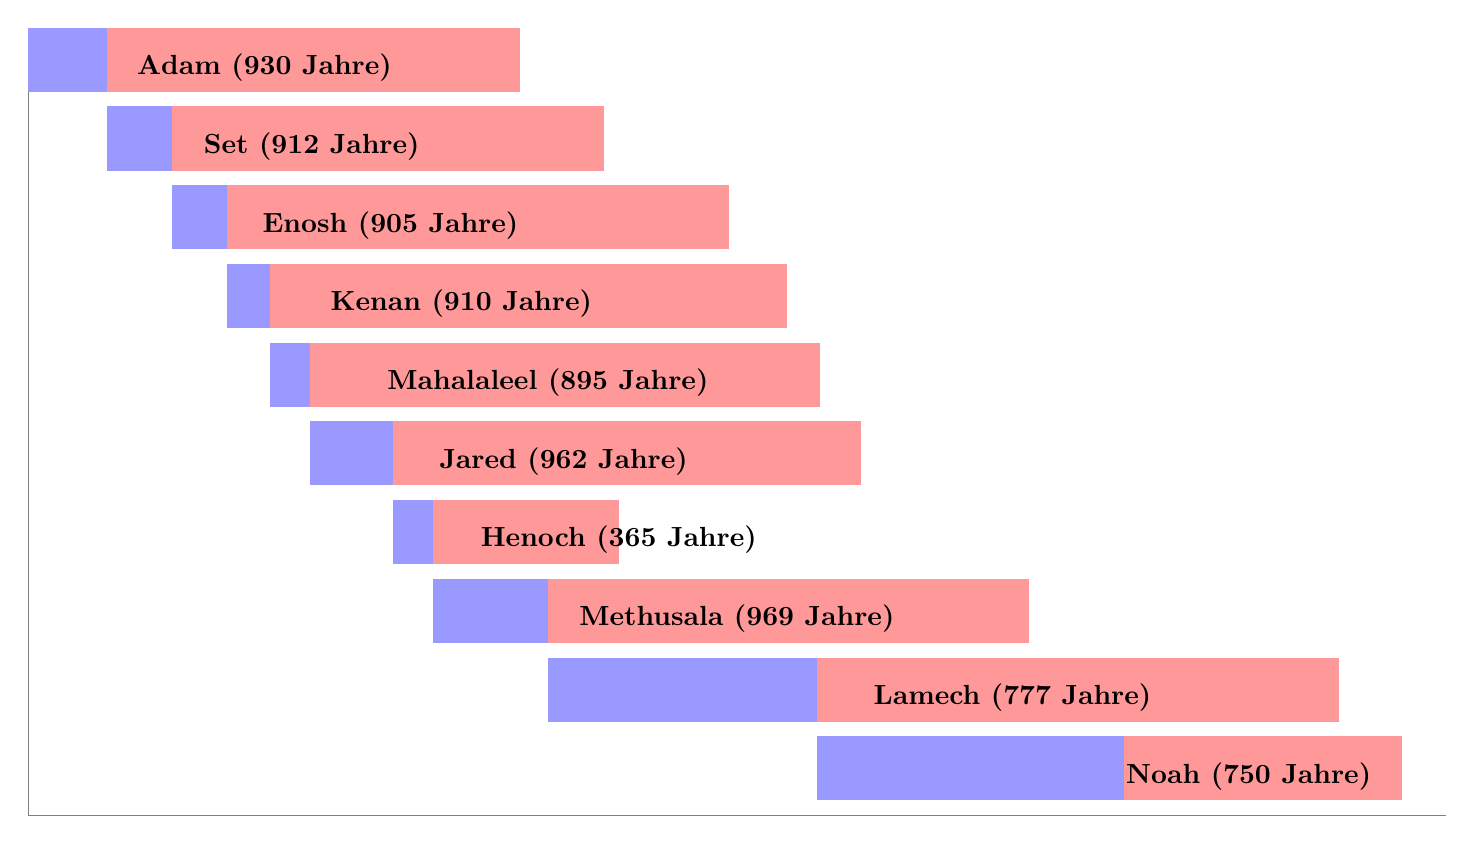
\begin{tikzpicture}		
		\draw[gray] (0,0) -- (0mm, 100mm);
		%Adam 130-800 (10.1 - 62.4)
		\filldraw[blue!40] (0,100mm) rectangle(10.1mm,92mm);
		\filldraw[red!40] (10.1mm,100mm) rectangle(62.4mm,92mm) node at (30mm, 92mm) [right, above, black]{\textbf{Adam (930 Jahre)}};	
		%Set 105-807 (8.19 - 62.9)
		\filldraw[blue!40] (10.1mm,90mm) rectangle(18.29mm,82mm);
		\filldraw[red!40] (18.29mm,90mm) rectangle(73.0mm,82mm) node at (36mm, 82mm) [right, above, black]{\textbf{Set (912 Jahre)}};
		%Enosch 90 - 815 (7.02 - 63.6)	
		\filldraw[blue!40] (18.29mm,80mm) rectangle (25.31mm,72mm);
		\filldraw[red!40] (25.31mm,80mm) rectangle(88.91mm,72mm) node at (46mm, 72mm) [right, above, black]{\textbf{Enosh (905 Jahre)}};
		%Kenan 70 - 840 (5.46 - 65.52)		
		\filldraw[blue!40] (25.31mm,70mm) rectangle(30.77mm,62mm);
		\filldraw[red!40] (30.77mm,70mm) rectangle(96.29mm,62mm) node at (55mm, 62mm) [right, above, black]{\textbf{Kenan (910 Jahre)}};
		%Mahalaleel 65 - 830 (5.07 - 64.7)
		\filldraw[blue!40] (30.77mm,60mm) rectangle(35.84mm,52mm);
		\filldraw[red!40] (35.84mm,60mm) rectangle(100.54mm,52mm) node at (66mm, 52mm) [right, above, black]{\textbf{Mahalaleel (895 Jahre)}};
		%Jared 162 - 800 (12.6 - 62.4)
		\filldraw[blue!40] (35.84mm,50mm) rectangle(46.44mm,42mm);
		\filldraw[red!40] (46.44mm,50mm) rectangle(105.68mm,42mm) node at (68mm, 42mm) [right, above, black]{\textbf{Jared (962 Jahre)}};
		%Henoch 65 - 300 (5.07 - 23.4)
		\filldraw[blue!40] (46.44mm,40mm) rectangle(51.51mm,32mm);
		\filldraw[red!40] (51.51mm,40mm) rectangle(74.91mm,32mm) node at (75mm, 32mm) [right, above, black]{\textbf{Henoch (365 Jahre)}};
		%Methusalah 187 - 782 (14.58 - 60.99)
		\filldraw[blue!40] (51.51mm,30mm) rectangle(66.09mm,22mm);
		\filldraw[red!40] (66.09mm,30mm) rectangle(127.08mm,22mm) node at (90mm, 22mm) [right, above, black]{\textbf{Methusala (969 Jahre)}};
		%Lamech 182 - 595 (14.19 - 46.41)
		\filldraw[blue!40] (66.09mm,20mm) rectangle(100.28mm,12mm);
		\filldraw[red!40] (100.28mm,20mm) rectangle(166.37mm,12mm) node at (125mm, 12mm) [right, above, black]{\textbf{Lamech (777 Jahre)}};
		% Noah 500 - 450 (39 - 35.1)
		\filldraw[blue!40] (100.28mm,10mm) rectangle(139.28mm,2mm);
		\filldraw[red!40] (139.28mm,10mm) rectangle(174.38mm,2mm) node at (155mm, 2mm) [right, above, black]{\textbf{Noah (750 Jahre)}};
		
		\draw[gray] (0,0) -- (180mm, 0mm);
	\end{tikzpicture}		
	\caption{Lebensjahre bis Noah}
	\label{balken_alter}
\end{figure}
In diesem Kapitel wird das Geschlechtsregister Adams bis Noah aufgelistet. Die Menschen wurden zu der Zeit ziemlich alt. Durch dieses Alter gab es eine Spezielle konstellation.
Es ist interessant zu sehen (Abbildung: \ref{balken_alter}), wie Noah noch die Geburt von Lamech knapp miterleben konnte. Ich glaube zwar nicht, dass die sich nach so langer Zeit noch gekannt haben, aber es ist spannend. Am Ende das blauen Balken wurde dann der erste Sohn geboren, oder wenigsten die Person die die direkte Linie zu Jesus weiter führte. 
Dieses Kapitel endet mit der Erwähnung von Noah und es werden seine Söhne Sem, Ham, Japhet aufgelistet.
    
\subsubsection{1. Mose 6 (Genesis 6)}
Am Anfang des Kapitels wird erklärt, warum Gott die Menschen vernichten wollte. Es steht nirgends, dass er die Erde vernichten will, sondern nur die Lebewesen auf dieser Erde. Gott fand, das alle Menschen schlecht sind. In Vers 6 steht folgendes.
\begin{bibeltext}{ELB}{Gen}{6:6}
	Und es reute den \herr , dass er den Menschen gemacht hatte auf der Erde, und es schmerzte ihn in sein Herz hinein.
\end{bibeltext}
In Vers 7 steht, dass er nicht nur die Menschen vernichten will sondern auch alle Tier auf dieser Erde. Und dann in Vers 8.
\begin{bibeltext}{ELB}{Gen}{6:7}
	Noah aber fand Gnade in den Augen des Herrn.
\end{bibeltext}
Auf der ganzen Erde nur ein Mann. Dieser eine Mann wird als gerechter und vollkommener Mann unter seinen Zeitgenossen dargestellt. Durch diesen gerechten Menschen wurden dann auch die Tier nach ihrer Art gerettet. Für die Rettung der Menschen und der Tiere gab ihm Gott den Auftrag ein Schiff zu bauen. Mit dem Schiff und dem Regen fängt eine Geschichte an, die mit der Wiederkunft Jesus im neuen Testament vergleichbar ist. Nur mit einer Sintflut und einem grossen Schiff, kann so eine parallele zu unserer heutigen Zeit unsere Erlösung mit Jesus Christus bildlich dargestellt werden.
\begin{figure}[h]
	\begin{tabular}{lcl}
		Schiff & = & Jesus\\
		Wasser & = & ungläuber Mensch\\
		Noah & = & gläubige Mensch\\
	\end{tabular}
\end{figure}
Noah hat Gott gehorcht und das Schiff gebaut. Die restliche Menschheit wollte sich nicht von einem Gott etwas sagen lassen. Da sind wir schlauer. Uns geht es ja gut, für was brauchen wir noch einen Gott? Sollen wir und die Mühe machen und ein Schiff zusammen zimmern? Läuft doch alles so prima. Eines Tages fing es an zu regnen. Naja ein bisschen Regen wieso sich Sorgen machen. Der Regen wurde aber immer schlimmer.

Das passiert doch auch heute. Mehr Überschwemmungn, mehr Krankheiten, mehr Unruhen und Unzufriedenheit in der Menschheit. Perpektivlosigkeiten, werden mit Versuchen den Weltraum zu ergründen überbrückt. Von Menschen gemachter Klimawandel? Vielleicht ist es auch ein von Gott gemachter Klimawandel und es geht wie in der Offenbarung beschrieben langsam dem Ende entgegen? Outet man sich als Christ, wird man ausgelacht. \textbf{Wir} haben alles im Griff. \textbf{Wir} brauchen niemand, ein bisschen CO\textsuperscript{2} weniger in die Luft jagen und schon wird es uns wieder besser gehen. Kann sein, dass es so wird, muss aber nicht. Es kann aber auch wie zu Noahs Zeiten werden, dass wir besser auf Jesus vertrauen sollten und so in die Arche gelangen um gerettet zu werden.
    %\subsubsection{1. Mose 7 (Genesis 7)}
    %\input{Kurs/bibelkommentar/1_Moses/8.tex}
    %\subsection{Kapitel 9}

Jetzt nachdem sie die Arche verlassen haben und wieder an Land sind, segnet Gott Noah und seine Söhne. Als erstes sollen sie sich wieder vermehren und die Erde bevölkern. Das Töten war in der Urfassung der Schöpfung nicht vorgesehen. Hier stellt Gott alles was auf der Erde lebt den Menschen Untertan. 

    %\input{Kurs/bibelkommentar/1_Moses/10.tex}
%%%%%%%%%%%%%%%%%%%%%%%%%%%%%%%%%%%%%%%%%%%%%%%%%%%%%%%%%%%%%%%%%%%%%%%%%%%%%%%%%%%%%%%%%%%%%%%%%%%%%
%%%%%%%%%  2. Mose
%%%%%%%%%%%%%%%%%%%%%%%%%%%%%%%%%%%%%%%%%%%%%%%%%%%%%%%%%%%%%%%%%%%%%%%%%%%%%%%%%%%%%%%%%%%%%%%%%%%%%
\section{Allgemeines zum Buch 2. Mose (Exodus)}
\subsection{WER?}
\subsection{WEM?}
\subsection{WANN?}
\subsection{WAS?}
\subsection{WIE?}
\subsection{Übersichtsfragen zu 2. bis 5. Mose}
    
\begin{enumerate}
    \item \textbf{Warum wird 2. Mose auch das «Buch der Erlösung» genannt?}\\
    Es zeigt die Befreiung Israels aus der Knechtschaft Ägyptens durch das Blut eines Lammes. Durch die zehn Gebote wird Gottes Willen und Heiligkeit weiter offenbart. Aber kein Mensch ist fähig diese zehn Gebote vollständig einzuhalten. Gott zeigt uns einen Ausweg durch den Weg und Dienst in der Stiftshütte. Dies ist ein wunderbarer Prohetischer hinweis aus auf den Erlöser Jesus Christus. In 2. Mose bedeutet Erlösung auch: Wiederherstellung und ganz machen. Gott macht aus einer Familie ein Volk, gibt ihnen eine Regierung, ein Gottesdienst, ein Gesetz und bestätigt ein Land. So erlöst Gott und stellt es unter seine Leitung und Fürsorge.
    \item \textbf{Worauf weist der hebräiche Titel von 3. Mode, Leviticus, hin?}\\
    Auf die Aufgabe der Priester und Leviten. Gott beruft sie in Seinen Dienst. Gott zeigt dem Volk durch den Dienst und die Aufgaben der Priester sowie durch die entsprechenden Opfer den WEg zur Gemeinschaft mit Ihm. Damit wird deutlich, dass Gottes Einladung gilt: das Volk Israel kann kommen. Jedosch nur auf dem von Ihm vorgezeichneten Weg. Dies erinnnert an die Aussage Jesu:
    \begin{bibeltext}{ELB}{Joh}{14:6}
        Ich bin der Weg, die Wahrheit und das Leben, niemand kommt zum Vater als nur durch Mich.
    \end{bibeltext}
    \item \textbf{Warum heisst 4. Mose auch "In der Wüste"?}
    Gott hat Sein Volk mit starker Hand erlöst. Aus Ihnen ein Volk geformt. Sich ihnen in wunderbarer und herrlicher Weise offenbart. Doch Israel reagiert immer wieder mit Unglauben und Auflehnung, bis das "Fass überläuft", bis zum "Point of Return". Siehe:
    \begin{bibeltext}{Sch2}{Num}{14:11}
        Und der \herr{} sprach zu Mose: \flqq Wie lange noch will mich dieses Volk verachten? Und wie lange noch wollen sie nicht an mich glauben, trotz aller Zeichen, die ich unter ihnen getan habe?\frqq{}
    \end{bibeltext}
    \begin{bibeltext}{Sch2}{Num}{14:16-22}
        Weil der \herr{} dieses Volk nicht in das Land bringen konnte, das er ihnen zugeschworen hatte, darum hat er sie in der Wüste hingeschlachtet! So lass nun die Macht des \herr n gross werden, wie du gesprochen und verheissen hast: \flqq Der \herr{} ist langsam zum Zorn und gross an der Gnade; er vergibt Schuld und Übertretungen, obgleich er keineswegs ungestraft lässt, sondern die Schuld der Väter heisucht an den Kindern, bis in das dritte und vierte Glied. Vergib nun die Schuld dieses Volkes nach deiner grossen Gnade, wie du auch diesem Volk verziehen hast non Ägypten an bis hierher.\frqq{}

        Da sprach der \herr : Ich habe vergeben nach deinem Wort. Aber - so war ich lebe und die ganze Erde mit der Herrlichkeit des \herr n erfüllt werden soll. Keiner der Männer, die meine Herrlichkeit und meine Zeichen gesehen haben, die ich in Ägypten und in der Wüste getan habe, und die mich nun schon zehnmal versucht und meiner Stimme nicht gehorcht haben.
    \end{bibeltext}
    Entsprechend beginnt eine 40-jährige Wüstenwanderung voller Not und Elend, bis alle, die Gottes Wege verwarfen, in der Wüste starben und somit das Land der Verheissung nicht zu sehen bekamen.
    \item \textbf{Warum ist die hebräische Bezeichnung Devarim, übersetzt "Wort", für 5. Mose treffend?}
    Im Griechischen wird 5. Mose "Deutoronium" genannt, übersetzt "Zweites Gesetz". Eigentlich ein unglücklicher Name, denn es ist kein zweites Gesetz, sondern der Rückblick eines alt gewordenen Mannes. Mose ist zu dieser Zeit mindestens doppelt so alt wie die ältesten Israeliten (Ausnahme Kaleb und Josua). Er lässt sein Leben Revue passieren. Ein Leben voll Abenteuer, Segen, Bewahrung, Leid und menschliches Versagens. Docj über allem stand immer die Treue unf Grösse Gottes. In 5. Mose erinnert Mose "seine Enkel" noch einmal an alle Wundertaten Gottes, an Seine Bestimmungen und an Sein Gesetz. Dabei motiviert er das Volk bei seinem Gott zu bleiben und Gottes Anordungen Folge zu leisten.

    Gleichzeitig richtet er ihr Augenmerk auch hin in die ferne Zukunft, indem er sagt:
    \begin{bibeltext}{Sch2}{Deu}{18:5}
        Einen Propheten wie mich wir der \herr , dein Gott, dir erwecken aus dir und aus deinen Brüdern; dem sollt ihr gehorchen.
    \end{bibeltext}
    Damit zeigt Mose, dass die 5 Bücher Mose nicht das Ende, sondern der Anfang der Erlösung ist, \textbf{dessen Zielkoordinaten sich in Jesus Christus treffen.}

\end{enumerate}
\subsection{Persönliche Kapitel Kommentare}
    \subsubsection{2. Mose 1 (Exodus 1)}
%%%%%%%%%%%%%%%%%%%%%%%%%%%%%%%%%%%%%%%%%%%%%%%%%%%%%%%%%%%%%%%%%%%%%%%%%%%%%%%%%%%%%%%%%%%%%%%%%%%%%
%%%%%%%% 3. Mose
%%%%%%%%%%%%%%%%%%%%%%%%%%%%%%%%%%%%%%%%%%%%%%%%%%%%%%%%%%%%%%%%%%%%%%%%%%%%%%%%%%%%%%%%%%%%%%%%%%%%%
\section{Allgemeines zum Buch 3. Mose (Levitikus)}
\subsection{WER?}
\subsection{WEM?}
\subsection{WANN?}
\subsection{WAS?}
\subsection{WIE?}
\subsection{Übersichtsfragen zu 3. Mose}
    \section{Übersichtsfragen zu 3. Mose}
\begin{enumerate}
    \item Worauf weist der hebräische Titel von 3. Mose, Leviticus, hin?\\
    Auf die Aufgabe der Priester und Leviten. Gott beruft sie in Seinen Dienst. Gott zeigt dem Volk durch den Dienst und die Aufgaben der Priester sowie durch die entsprechenden Opfer den Weg zur Gemeinschaft mit Ihm. Damit wird deutlich, dass Gottes Einladung gilt: das Volk Israel kann kommen. Jedoch nur auf dem von Ihm vorgezeichneten Weg. Dies erinnert an die Aussage Jesu:
\begin{bibeltext}{Sch2}{Joh}{14:6}
    Jesus spricht zu ihm: Ich bin der Weg und die Wahrheit und das Leben; niemand kommt zum Vater als nur durch mich!
\end{bibeltext}
\end{enumerate}
\subsection{Persönliche Kapitel Kommentare}
%%%%%%%%%%%%%%%%%%%%%%%%%%%%%%%%%%%%%%%%%%%%%%%%%%%%%%%%%%%%%%%%%%%%%%%%%%%%%%%%%%%%%%%%%%%%%%%%%%%%%
%%%%%%%% 4. Mose
%%%%%%%%%%%%%%%%%%%%%%%%%%%%%%%%%%%%%%%%%%%%%%%%%%%%%%%%%%%%%%%%%%%%%%%%%%%%%%%%%%%%%%%%%%%%%%%%%%%%%
\section{Allgemeines zum Buch 4. Mose (Numeri)}
\subsection{WER?}
\subsection{WEM?}
\subsection{WANN?}
\subsection{WAS?}
\subsection{WIE?}
\subsection{Übersichtsfragen zu 4. Mose}
    \section{Übersichtsfragen zu 4. Mose}
\begin{enumerate}
    \item textbf{Warum heisst 4. Mose auch «In der Wüste»?}\\
    Gott hat sein Volk mit starker Hand erlöst. Aus ihnen ein Volk geformt. Sich ihnen und wunderbarer und herrlicher Weise offenbart. Doch Isreal reagiert immer wieder in Unglauben und in Auflehnung bis das \flqq bis das Fass überläuft \frqq, bis zum \flqq Point of no return \frqq.
    \begin{bibeltext}{Sch2}{Num}{14:11}
        Und der \herr sprach zu Mose: Wie lange noch will mich dieses Volk verachten? Und wie lange noch wollen, sie nicht an mich glauben, trotz aller Zeichen, die ich unter ihnen getan habe?
    \end{bibeltext}
    \begin{bibeltext}{Sch2}{Num}{14:22-23}
        Keiner der Männer die meine Herrlichkeit und meine Zeichen gesehen haben, die ich in Ägypten und in der Wüste getan habe, und die mich nun schon zehnmal versucht und meiner Stimme nicht gehorcht haben, soll das Land sehen, das ich ihren Vätern zugeschworen habe; ja keiner soll es sehen, der micht verachtet hat!
    \end{bibeltext}
    Entsprechent beginnt eine 40jährige Wüstenwanderung, voll Not und Elend, bis alle, Gottes Wege verwarfen, in der Wüsten starben und somit das Land der Verheissung nicht zu sehen bekamen.
\end{enumerate}
\subsection{Persönliche Kapitel Kommentare}
%%%%%%%%%%%%%%%%%%%%%%%%%%%%%%%%%%%%%%%%%%%%%%%%%%%%%%%%%%%%%%%%%%%%%%%%%%%%%%%%%%%%%%%%%%%%%%%%%%%%%
%%%%%%%% 5. Mose
%%%%%%%%%%%%%%%%%%%%%%%%%%%%%%%%%%%%%%%%%%%%%%%%%%%%%%%%%%%%%%%%%%%%%%%%%%%%%%%%%%%%%%%%%%%%%%%%%%%%%
\section{Allgemeines zum Buch 5. Mose (Deuteronomium)}
\subsection{WER?}
\subsection{WEM?}
\subsection{WANN?}
\subsection{WAS?}
\subsection{WIE?}
\subsection{Übersichtsfragen zu 5. Mose}
    \section{Übersichtsfragen zu 5. Mose}
\begin{enumerate}
    \item Warum ist die hebräische Bezeichnung Devarim, übersetzt «Worte», für 5. Mose treffend?\\
    Im Griechischen wird 5. Mose \flqq Deuteronomium\frqq{} genannt, übersetzt \flqq Zweites Gesetz\frqq . Eigentlich ein unglücklicher Name, denn es ist kein zweites Gesetz, sondern der Rückblick eines alt gewordenen Mannes. Mose ist zu dieser Zeit mindestens doppelt so alt wie die ältesten Israeliten (mit ausnahme von Josua und Kaleb). Er lässt sein Leben Revue passieren. Ein Leben voll Abenteuer, Segen, Bewahrung, Leid und menschliches Versagens. Doch über allem stand immer die Treue und Grösse Gottes. In 5. Mose erinnert Mose seine Enkel noch einmal an alle Wundertaten Gottes, an Seine Bestimmungen und an Sein Gesetz. Dabei motiviert er das Volk bei seinem Gott zu bleiben und Gottes Anordnungen Folge zu leisten. Gleichzeitig richtet er ihr Augenmerk auch hin in die ferne Zukunft, indem er sagt: ""
    \begin{bibeltext}{Sch2}{Deut}{18:15}
        Einen Propheten wie mich wird dir der \herr, dein Gott, erwecken aus deiner Mitte, aus deinen Brüdern; auf ihn sollst du hören!
    \end{bibeltext}
    Damit zeigt Mose, dass die 5 Bücher Mose nicht das Ende, sondern der Anfang der Erlösung ist, dessen Zielkoordinaten sich in Jesus Christus treffen.
\end{enumerate}
\subsection{Persönliche Kapitel Kommentare}
%%%%%%%%%%%%%%%%%%%%%%%%%%%%%%%%%%%%%%%%%%%%%%%%%%%%%%%%%%%%%%%%%%%%%%%%%%%%%%%%%%%%%%%%%%%%%%%%%%%%%
%%%%%%%% Josua
%%%%%%%%%%%%%%%%%%%%%%%%%%%%%%%%%%%%%%%%%%%%%%%%%%%%%%%%%%%%%%%%%%%%%%%%%%%%%%%%%%%%%%%%%%%%%%%%%%%%%
\section{Allgemeines zum Buch Josua}
\subsection{WER?}
\subsection{WEM?}
\subsection{WANN?}
\subsection{WAS?}
\subsection{WIE?}
\subsection{Übersichtsfragen zu Josua}
    \section{Übersichtsfragen zu 1. und 2. Samuel}
\begin{enumerate}
    \item textbf{Wie hiess der letzte Richter?}\\
    Der letzte Richter wae Samuel. Die Israeliten wollten jetzt eine König wie alle anderen Völker rund um sie auch einen haben.
    \item textbf{Wie hiessen die beiden Könige unter Samuel?}\\
    Samuel hat dann unter protest zwei Könige gesalbt. Zuerst Saul, der nicht Gottes sondern seine eigenen Wege gehen wollt. Dann wurde noch während der Regierungszeit Sauls David zum König gesalbt.
    \item textbf{Welchen Einfluss hatte die Bundeslade auf Israel und die Philister?}
    Auf Israel: Keinen. Die Bundeslade wurde nur noch als Mittel zum zweck benutzt. War Krieg sollte die Lade sie beschützen.

    Auf die Philister, hatte die Lade eine verherende Auswirkung. Ihnen zeigte sich Gott als einzig wahren Gott. Ihre Götter vielen vor der Lade um. Es brach in dem Ort der Bundeslade Krankeit und Seuchen aus.
    \item textbf{Welches waren die politischen und geistlichen Höhepunkte unter David?}
    Ruhe von allen Feinden rings um Israel. Jerusalem wurde zur Hauptstadt Israels. Ausserdem hat er den Tempelbau vorbereitet. Selber sollte er den Tempel nicht mehr bauen sondern Sohn Salomon sollte dies tun:
    \begin{bibeltext}{Sch2}{1Sam}{7.12}
        Wenn deine Tage erfüllt sind und du bei deinen Vätern liegst, so will ich deinen Samen nach dir erwecken, der aus deinem Leib kommen wird, und ich werde sein Königtum befestigen. Der wird meinem Namen ein Haus bauen, und ich werde den Thron seines Königreichs auf ewig befestigen.
    \end{bibeltext}
    \item textbf{Wie hiessen die beiden herausragenden     Sünden im Leben Davids und die daraus folgenden Gerichte Gottes?}
    Der Ehebruch mit Bathseba und die Ermordung von Uria dem Ehemann der Bathseba
\end{enumerate}
\subsection{Persönliche Kapitel Kommentare}
%%%%%%%%%%%%%%%%%%%%%%%%%%%%%%%%%%%%%%%%%%%%%%%%%%%%%%%%%%%%%%%%%%%%%%%%%%%%%%%%%%%%%%%%%%%%%%%%%%%%%
%%%%%%%% 1. und 2. Samuel
%%%%%%%%%%%%%%%%%%%%%%%%%%%%%%%%%%%%%%%%%%%%%%%%%%%%%%%%%%%%%%%%%%%%%%%%%%%%%%%%%%%%%%%%%%%%%%%%%%%%%
\section{Allgemeines zum Buch 1. und 2. Samuel}
\subsection{WER?}
\subsection{WEM?}
\subsection{WANN?}
\subsection{WAS?}
\subsection{WIE?}
\subsection{Übersichtsfragen zu 1. und 2. Samuel}
    \section{Übersichtsfragen zu 1. und 2. Samuel}
\begin{enumerate}
    \item textbf{Wie hiess der letzte Richter?}\\
    Der letzte Richter wae Samuel. Die Israeliten wollten jetzt eine König wie alle anderen Völker rund um sie auch einen haben.
    \item textbf{Wie hiessen die beiden Könige unter Samuel?}\\
    Samuel hat dann unter protest zwei Könige gesalbt. Zuerst Saul, der nicht Gottes sondern seine eigenen Wege gehen wollt. Dann wurde noch während der Regierungszeit Sauls David zum König gesalbt.
    \item textbf{Welchen Einfluss hatte die Bundeslade auf Israel und die Philister?}
    Auf Israel: Keinen. Die Bundeslade wurde nur noch als Mittel zum zweck benutzt. War Krieg sollte die Lade sie beschützen.

    Auf die Philister, hatte die Lade eine verherende Auswirkung. Ihnen zeigte sich Gott als einzig wahren Gott. Ihre Götter vielen vor der Lade um. Es brach in dem Ort der Bundeslade Krankeit und Seuchen aus.
    \item textbf{Welches waren die politischen und geistlichen Höhepunkte unter David?}
    Ruhe von allen Feinden rings um Israel. Jerusalem wurde zur Hauptstadt Israels. Ausserdem hat er den Tempelbau vorbereitet. Selber sollte er den Tempel nicht mehr bauen sondern Sohn Salomon sollte dies tun:
    \begin{bibeltext}{Sch2}{1Sam}{7.12}
        Wenn deine Tage erfüllt sind und du bei deinen Vätern liegst, so will ich deinen Samen nach dir erwecken, der aus deinem Leib kommen wird, und ich werde sein Königtum befestigen. Der wird meinem Namen ein Haus bauen, und ich werde den Thron seines Königreichs auf ewig befestigen.
    \end{bibeltext}
    \item textbf{Wie hiessen die beiden herausragenden     Sünden im Leben Davids und die daraus folgenden Gerichte Gottes?}
    Der Ehebruch mit Bathseba und die Ermordung von Uria dem Ehemann der Bathseba
\end{enumerate}
\subsection{Persönliche Kapitel Kommentare}
%%%%%%%%%%%%%%%%%%%%%%%%%%%%%%%%%%%%%%%%%%%%%%%%%%%%%%%%%%%%%%%%%%%%%%%%%%%%%%%%%%%%%%%%%%%%%%%%%%%%%
%%%%%%%% 1. und 2. Könige
%%%%%%%%%%%%%%%%%%%%%%%%%%%%%%%%%%%%%%%%%%%%%%%%%%%%%%%%%%%%%%%%%%%%%%%%%%%%%%%%%%%%%%%%%%%%%%%%%%%%%
\section{Allgemeines zum Buch 1. und 2. Könige}
\subsection{WER?}
\subsection{WEM?}
\subsection{WANN?}
\subsection{WAS?}
\subsection{WIE?}
\subsection{Übersichtsfragen zu 1. und 2. Könige}
    \section{Übersichtsfragen zu 1. und 2. Samuel}
\begin{enumerate}
    \item textbf{Wie hiess der letzte Richter?}\\
    Der letzte Richter wae Samuel. Die Israeliten wollten jetzt eine König wie alle anderen Völker rund um sie auch einen haben.
    \item textbf{Wie hiessen die beiden Könige unter Samuel?}\\
    Samuel hat dann unter protest zwei Könige gesalbt. Zuerst Saul, der nicht Gottes sondern seine eigenen Wege gehen wollt. Dann wurde noch während der Regierungszeit Sauls David zum König gesalbt.
    \item textbf{Welchen Einfluss hatte die Bundeslade auf Israel und die Philister?}
    Auf Israel: Keinen. Die Bundeslade wurde nur noch als Mittel zum zweck benutzt. War Krieg sollte die Lade sie beschützen.

    Auf die Philister, hatte die Lade eine verherende Auswirkung. Ihnen zeigte sich Gott als einzig wahren Gott. Ihre Götter vielen vor der Lade um. Es brach in dem Ort der Bundeslade Krankeit und Seuchen aus.
    \item textbf{Welches waren die politischen und geistlichen Höhepunkte unter David?}
    Ruhe von allen Feinden rings um Israel. Jerusalem wurde zur Hauptstadt Israels. Ausserdem hat er den Tempelbau vorbereitet. Selber sollte er den Tempel nicht mehr bauen sondern Sohn Salomon sollte dies tun:
    \begin{bibeltext}{Sch2}{1Sam}{7.12}
        Wenn deine Tage erfüllt sind und du bei deinen Vätern liegst, so will ich deinen Samen nach dir erwecken, der aus deinem Leib kommen wird, und ich werde sein Königtum befestigen. Der wird meinem Namen ein Haus bauen, und ich werde den Thron seines Königreichs auf ewig befestigen.
    \end{bibeltext}
    \item textbf{Wie hiessen die beiden herausragenden     Sünden im Leben Davids und die daraus folgenden Gerichte Gottes?}
    Der Ehebruch mit Bathseba und die Ermordung von Uria dem Ehemann der Bathseba
\end{enumerate}
\subsection{Persönliche Kapitel Kommentare}
%%%%%%%%%%%%%%%%%%%%%%%%%%%%%%%%%%%%%%%%%%%%%%%%%%%%%%%%%%%%%%%%%%%%%%%%%%%%%%%%%%%%%%%%%%%%%%%%%%%%%
%%%%%%%% 1. und 2. Chronik
%%%%%%%%%%%%%%%%%%%%%%%%%%%%%%%%%%%%%%%%%%%%%%%%%%%%%%%%%%%%%%%%%%%%%%%%%%%%%%%%%%%%%%%%%%%%%%%%%%%%%
\section{Allgemeines zum Buch 1. und 2. Chronik}
\subsection{WER?}
\subsection{WEM?}
\subsection{WANN?}
\subsection{WAS?}
\subsection{WIE?}
\subsection{Übersichtsfragen zu 1. und 2. Chronik}
    \section{Übersichtsfragen zu 1. und 2. Könige}
\begin{enumerate}
    \item Fragen
\end{enumerate}
\subsection{Persönliche Kapitel Kommentare}
%%%%%%%%%%%%%%%%%%%%%%%%%%%%%%%%%%%%%%%%%%%%%%%%%%%%%%%%%%%%%%%%%%%%%%%%%%%%%%%%%%%%%%%%%%%%%%%%%%%%%
%%%%%%%% Hiob
%%%%%%%%%%%%%%%%%%%%%%%%%%%%%%%%%%%%%%%%%%%%%%%%%%%%%%%%%%%%%%%%%%%%%%%%%%%%%%%%%%%%%%%%%%%%%%%%%%%%%
\section{Allgemeines zum Buch Hiob}
\subsection{WER?}
\subsection{WEM?}
\subsection{WANN?}
\subsection{WAS?}
\subsection{WIE?}
\subsection{Übersichtsfragen zu Hiob}
    \subsection{Übersichtsfragen zu Hiob}
\begin{enumerate}
    \item \textbf{Wie lauten einige Charaktereigenschaften Hiobs}\\
    Untadelig, rechtschaffen, gottesfürchtig, geistlich gesinnt, keusch, hilfsbereit
    \item \textbf{Warum muss Hiob leiden?}\\
    Es tobt ein Kampf zwischen Gott und den Teufel. Der ist der Meinung, dass sobald es Hiob schlecht gehen wird dieser vom Glauben abfallen wird.
    \item \textbf{Wie lassen sich die ersten sechs Prüfungen Hiobs zusammenfassen?}\\
    Vernichtung seines gesamten Besitzes, Zerstörung seiner Gesundheit, Ratschlag seiner Ehefrau sich von Gott loszusagen und Selbstmord zu begehen.
     \item \textbf{Was führte zum Zerbruch von Hiob?}\\
     Die siebte Prüfung: Seine takt- und lieblosen, besserwisserischen und verurteilenden Freunde.
     \item \textbf{Was lernen wir aus dem Buch Hiob?}\\
     \begin{itemize}
     		\item Gott beanwortet nicht alle \flqq Warum-Fragen \frqq
     		\item Gott ist würdig, unabhängig von allen Lebensumstaänden angebetet zu werden
     \end{itemize}
     \item \textbf{Was bewirkt die grosse Wende?}\\
     Die Begegnung mit Gott, gefolgt von Busse und Beugung; das Gebet für seine Freunde war der Auslöser für vollständige Wiederherstellung.
     \item \textbf{Wo und wann fand die Geschichte Hiobs statt?}\\
     Im Land Uz, in Edom, was dem heutigen Jordanien entspricht, im 3. Jahrtausend vor Christus.
     
\end{enumerate}
\subsection{Persönliche Kapitel Kommentare}



